\documentclass[11pt]{article}
\usepackage[margin=0.85in]{geometry}
\usepackage{graphicx}
\usepackage{booktabs}
\usepackage{amsmath}
\usepackage{hyperref}

\title{BONE-MAP: A Resolution-Gated Open-Source Architecture for 3D Cortical Fracture Quantification and Multi-Modal Rehabilitation Tracking}
\date{}

\begin{document}
\maketitle

\begin{abstract}
\textbf{Purpose:} Rehabilitation following tibial fractures requires aligning 3D structural bone assessments with progressive weight-bearing milestones. However, automated bone-analysis tools frequently apply micro-CT trabecular algorithms to coarse clinical CT scans or report uncalibrated Hounsfield units (HU) as volumetric bone mineral density (BMD), creating physical reliability hazards.
\textbf{Methods:} We developed BONE-MAP, an open-source, resolution-gated architecture integrating TotalSegmentator appendicular segmentation, a CPU HU fallback, 3D Slicer label-map round-trip, fibula-referenced four-quadrant cortical bridging, and physiotherapy tracking (\%BW, active ROM, VAS, LEFS, clinician mRUST). Hard guardrails lock trabecular metrics above 0.25\,mm spacing and uncalibrated BMD. Validation spanned 18 clinical lower-limb CTs with 3D Slicer ground truth, 0.020\,mm micro-CT, and 186 tibial plateau fracture cases.
\textbf{Results:} Across all 18 CT limbs, TotalSegmentator outperformed the CPU fallback in Tibia Dice (median 0.9157 vs 0.7344, Wilcoxon $p=3.82\times 10^{-5}$) and HD95 (median 3.73 vs 16.14\,mm, $p=0.034$), reaching $0.9465\pm 0.0211$ Dice and $0.63\pm 0.15$\,mm ASSD on $\le 0.85$\,mm scans. Bland--Altman cortical thickness bias was $-0.029\pm 0.060$\,mm. Medial-ridge trabecular refinement cut 0.020\,mm micro-CT error from 0.1174\,mm to 0.0194\,mm (0.222 vs 0.2414\,mm reference).
\textbf{Conclusion:} BONE-MAP provides a reproducible, physically honest software baseline uniting multi-modal tibial morphometry with rehabilitation telemetry while preventing sub-resolution or uncalibrated metric fabrication.
\end{abstract}

\noindent\textbf{Keywords:} Tibial fracture; Cortical thickness; Resolution gate; TotalSegmentator; Physiotherapy rehabilitation.

\section{Introduction}
Long-bone fractures of the tibia---spanning high-energy diaphyseal trauma and intra-articular tibial plateau fractures---undergo prolonged secondary healing in which mechanical loading directly stimulates bone remodeling. In routine clinical workflows, structural imaging assessment and functional physiotherapy rehabilitation remain disconnected. Orthopedic and radiologic evaluations rely on qualitative CT slice inspection or ordinal radiographic scales such as RUST and Modified RUST (mRUST)~\cite{whelan2010rust,litrenta2015mrust}, while physiotherapists prescribe weight-bearing progression, active knee range of motion (ROM), pain visual analog scores (VAS), and Lower Extremity Functional Scale (LEFS) milestones~\cite{binkley1999lefs} without spatially resolved cortical wall thickness or quadrant-bridging metrics.

Existing quantitative imaging pipelines present two major pitfalls when applied to routine clinical care: (1) partial-volume blurring at clinical CT spacings (0.5--1.0\,mm) renders individual trabeculae unresolvable~\cite{whittier2020hrpqct}, and (2) converting single-energy Hounsfield units (HU) to volumetric BMD without an in-scan calibration phantom violates quantitative CT standards~\cite{engelke2008iscd}. We present BONE-MAP (code repository anonymized during double-blind peer review), an open-source imaging informatics platform integrating TotalSegmentator~\cite{wasserthal2023totalsegmentator}, SimpleITK~\cite{lowekamp2013simpleitk}, 3D Slicer round-trip editing~\cite{fedorov2012slicer}, physiotherapy telemetry, and strict physical guardrails.

\section{Materials and Methods}
\subsection{Architecture and Guardrailed Morphometry}
BONE-MAP links longitudinal encounters ($T_0\dots T_n$) across FastAPI/SQLite and Next.js/Three.js (Fig.~\ref{fig:arch}). Incoming volumes undergo PHI stripping, LPS canonical orientation, hardware exclusion ($\ge 2500$\,HU dilated ring), and dual segmentation via GPU TotalSegmentator (\texttt{appendicular\_bones}) or CPU HU morphology. Cortical thickness uses anisotropic 3D Euclidean Distance Transform (EDT) ridge core sampling ($\text{edt} \ge 0.45 \times \text{local\_ridge}$), SVD fragment alignment, and fibula-referenced four-quadrant polarity. Medullary trabecular analysis activates strictly at voxel spacing $\le 0.25$\,mm using refined 0.90-ridge core sampling calibrated toward Hildebrand--R\"uegsegger local thickness~\cite{hildebrand1997thickness}. Phantom-free HU values never emit volumetric BMD, and non-tibial OOD scans are excluded.

\begin{figure}[ht]
\centering
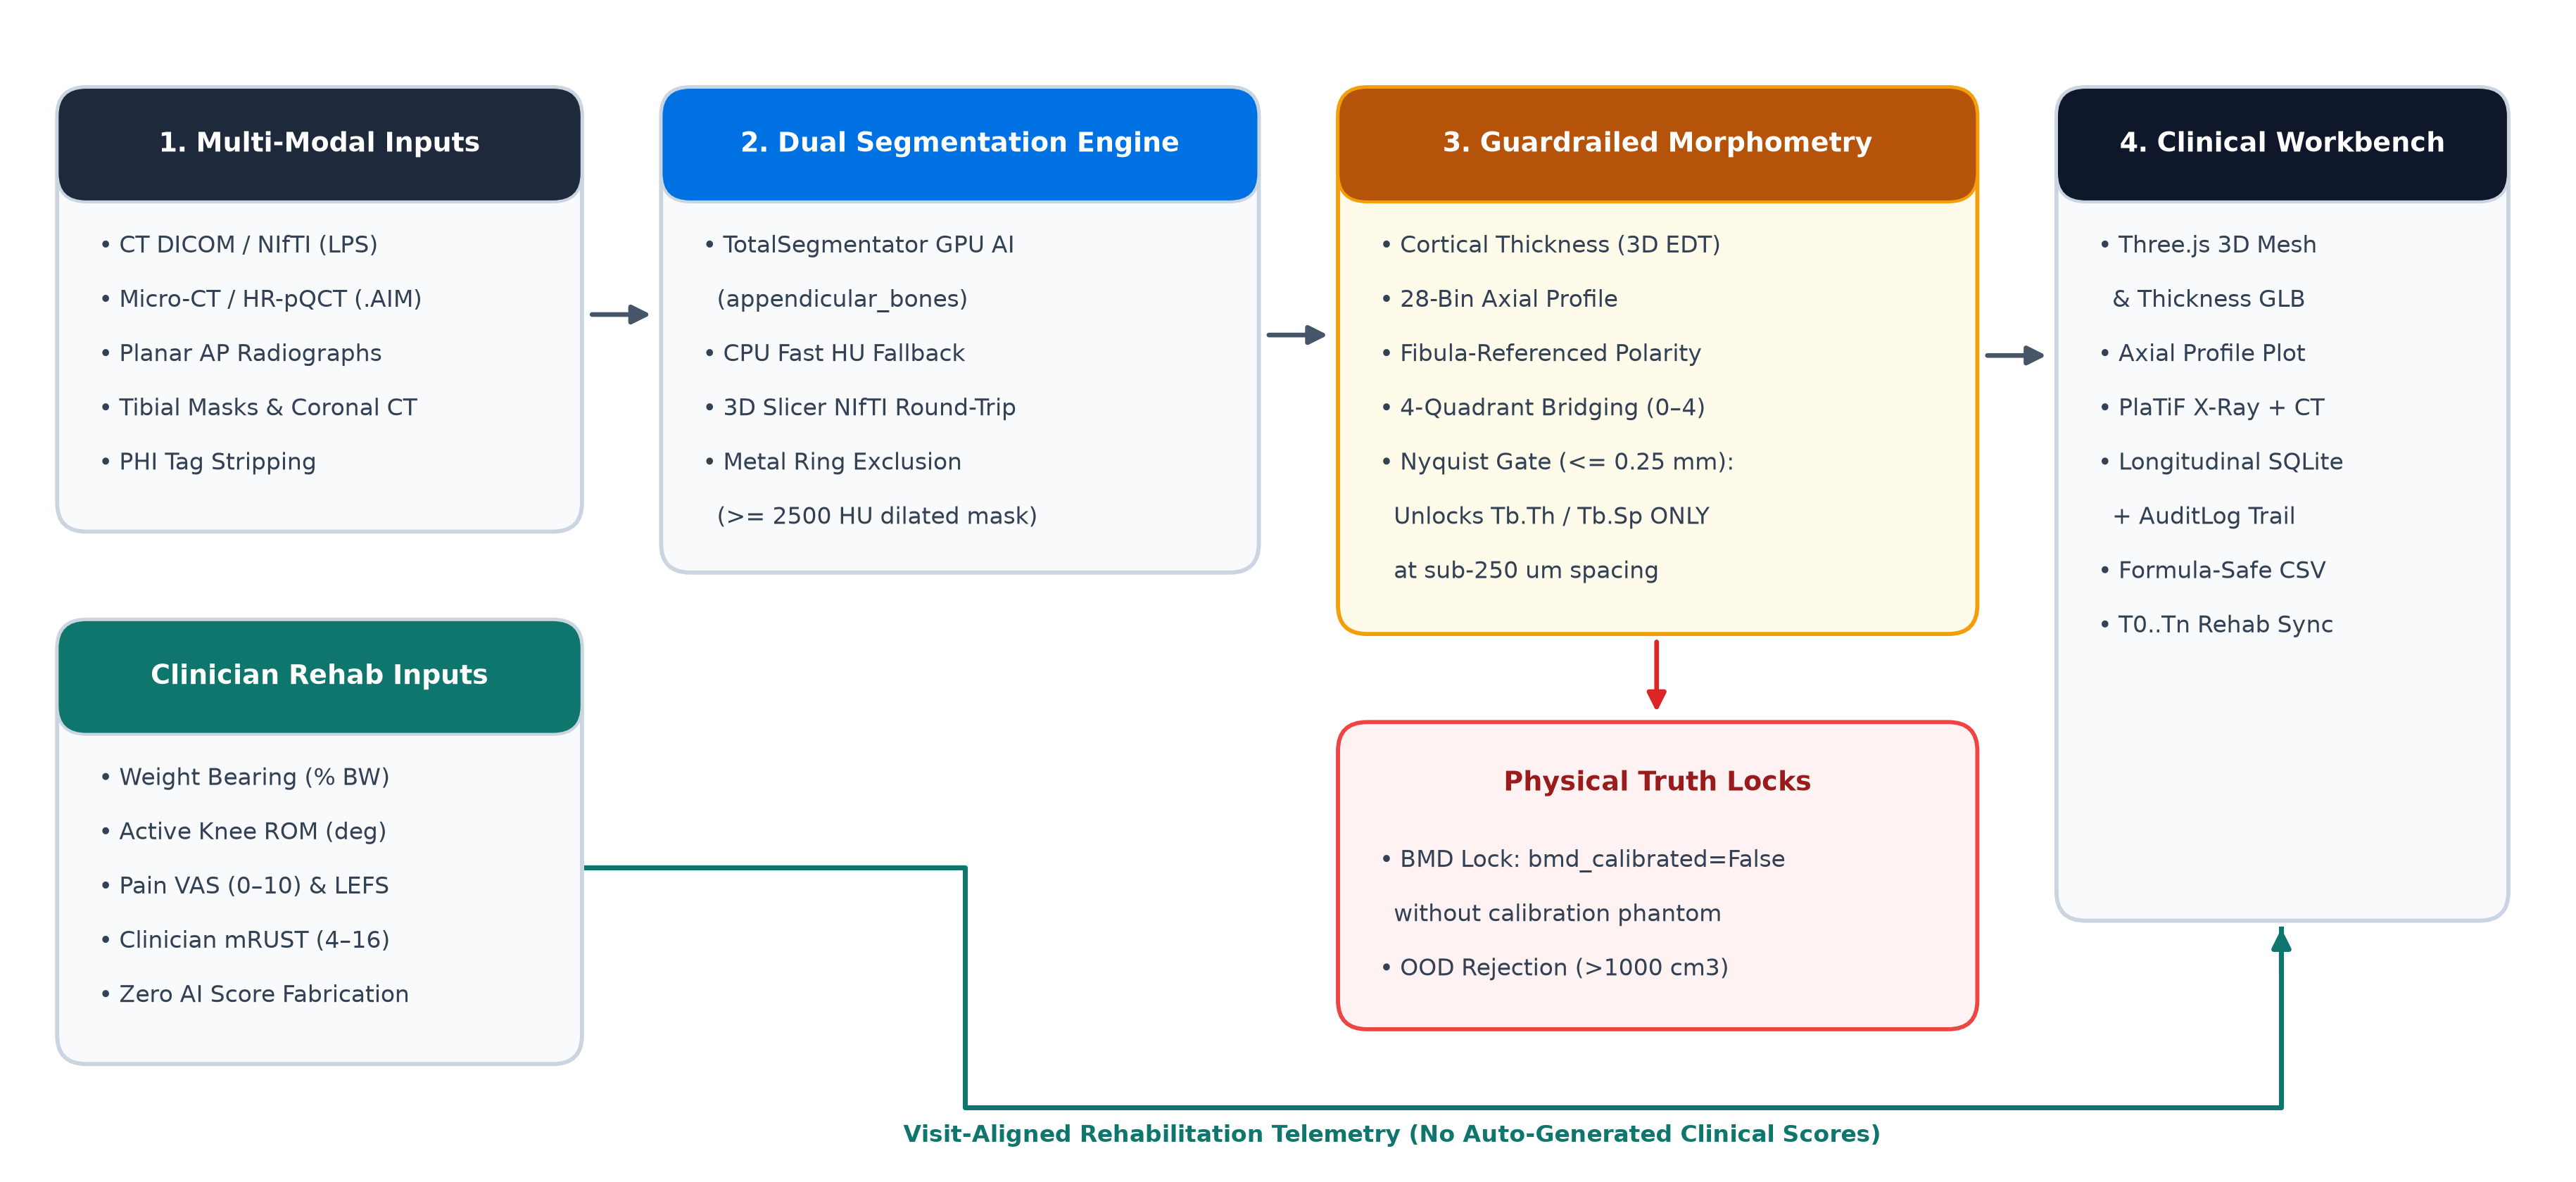
\includegraphics[width=\textwidth]{figures/fig1_architecture_pipeline.png}
\caption{End-to-end BONE-MAP architecture connecting multi-modal inputs, dual segmentation, physical truth guardrails, and rehabilitation telemetry.}
\label{fig:arch}
\end{figure}

\subsection{Public Multi-Cohort Evaluation}
Validation spanned four open-access Zenodo collections ($N=205$ total evaluations): 18 lower-limb CTs from VSDFullBody~\cite{vsdfullbody_zenodo} with resampled 3D Slicer ground truth stratified at $\le 0.85$\,mm ($n=10$) vs $>0.85$\,mm ($n=8$); ORMIR 0.020\,mm micro-CT \texttt{CHAR\_NOCMP\_020.AIM}~\cite{ormir_zenodo} with Scanco IPL sphere-fit reference (0.2414\,mm); all 186 tibial plateau patients in PlaTiF Parts 1--5~\cite{platif_zenodo}; and a PENGWIN26 pelvic fracture OOD control~\cite{pengwin_zenodo}.

\section{Results}
Across all 18 CT limbs (Table~\ref{tab:seg}, Fig.~\ref{fig:seg}), TotalSegmentator outperformed the CPU fallback in Tibia Dice (median 0.9157 vs 0.7344, $p=3.82\times 10^{-5}$) and HD95 (3.73 vs 16.14\,mm, $p=0.034$), reaching $0.9465\pm 0.0211$ Dice and $0.63\pm 0.15$\,mm ASSD on $\le 0.85$\,mm scans. Bland--Altman cortical thickness bias was $-0.0289\pm 0.0598$\,mm across all 18 limbs and $-0.0050\pm 0.0053$\,mm on standard CTs (Fig.~\ref{fig:ba}). On 0.020\,mm micro-CT (Fig.~\ref{fig:res}), medial-ridge refinement reduced error from 0.1174\,mm to 0.0194\,mm ($<1$ voxel). Across all 186 PlaTiF patients (Fig.~\ref{fig:platif}), 150 (80.6\%) included paired 2D coronal CT slices and expert tibia masks averaged $8.52\pm 2.71\%$ of radiograph FOV.

\begin{table}[ht]
\centering
\caption{3D tibia segmentation performance across 18 lower-limb CT volumes.}
\label{tab:seg}
\begin{tabular}{lcccc}
\toprule
Cohort \& Method & $n$ & Tibia Dice Mean $\pm$ SD & Median [IQR] & HD95 Med (mm) \\
\midrule
Pooled TotalSegmentator & 18 & $0.7630 \pm 0.2917$ & 0.9157 [0.649--0.948] & 3.73 \\
Pooled Fast HU & 18 & $0.4461 \pm 0.3941$ & 0.7344 [0.000--0.758] & 16.14 \\
Standard ($\le 0.85$\,mm) TotalSeg & 10 & $0.9465 \pm 0.0211$ & 0.9480 [0.931--0.965] & 1.59 \\
Coarse ($>0.85$\,mm) TotalSeg & 8 & $0.5338 \pm 0.3129$ & 0.6133 [0.412--0.749] & 9.66 \\
\bottomrule
\end{tabular}
\end{table}

\begin{figure}[ht]
\centering
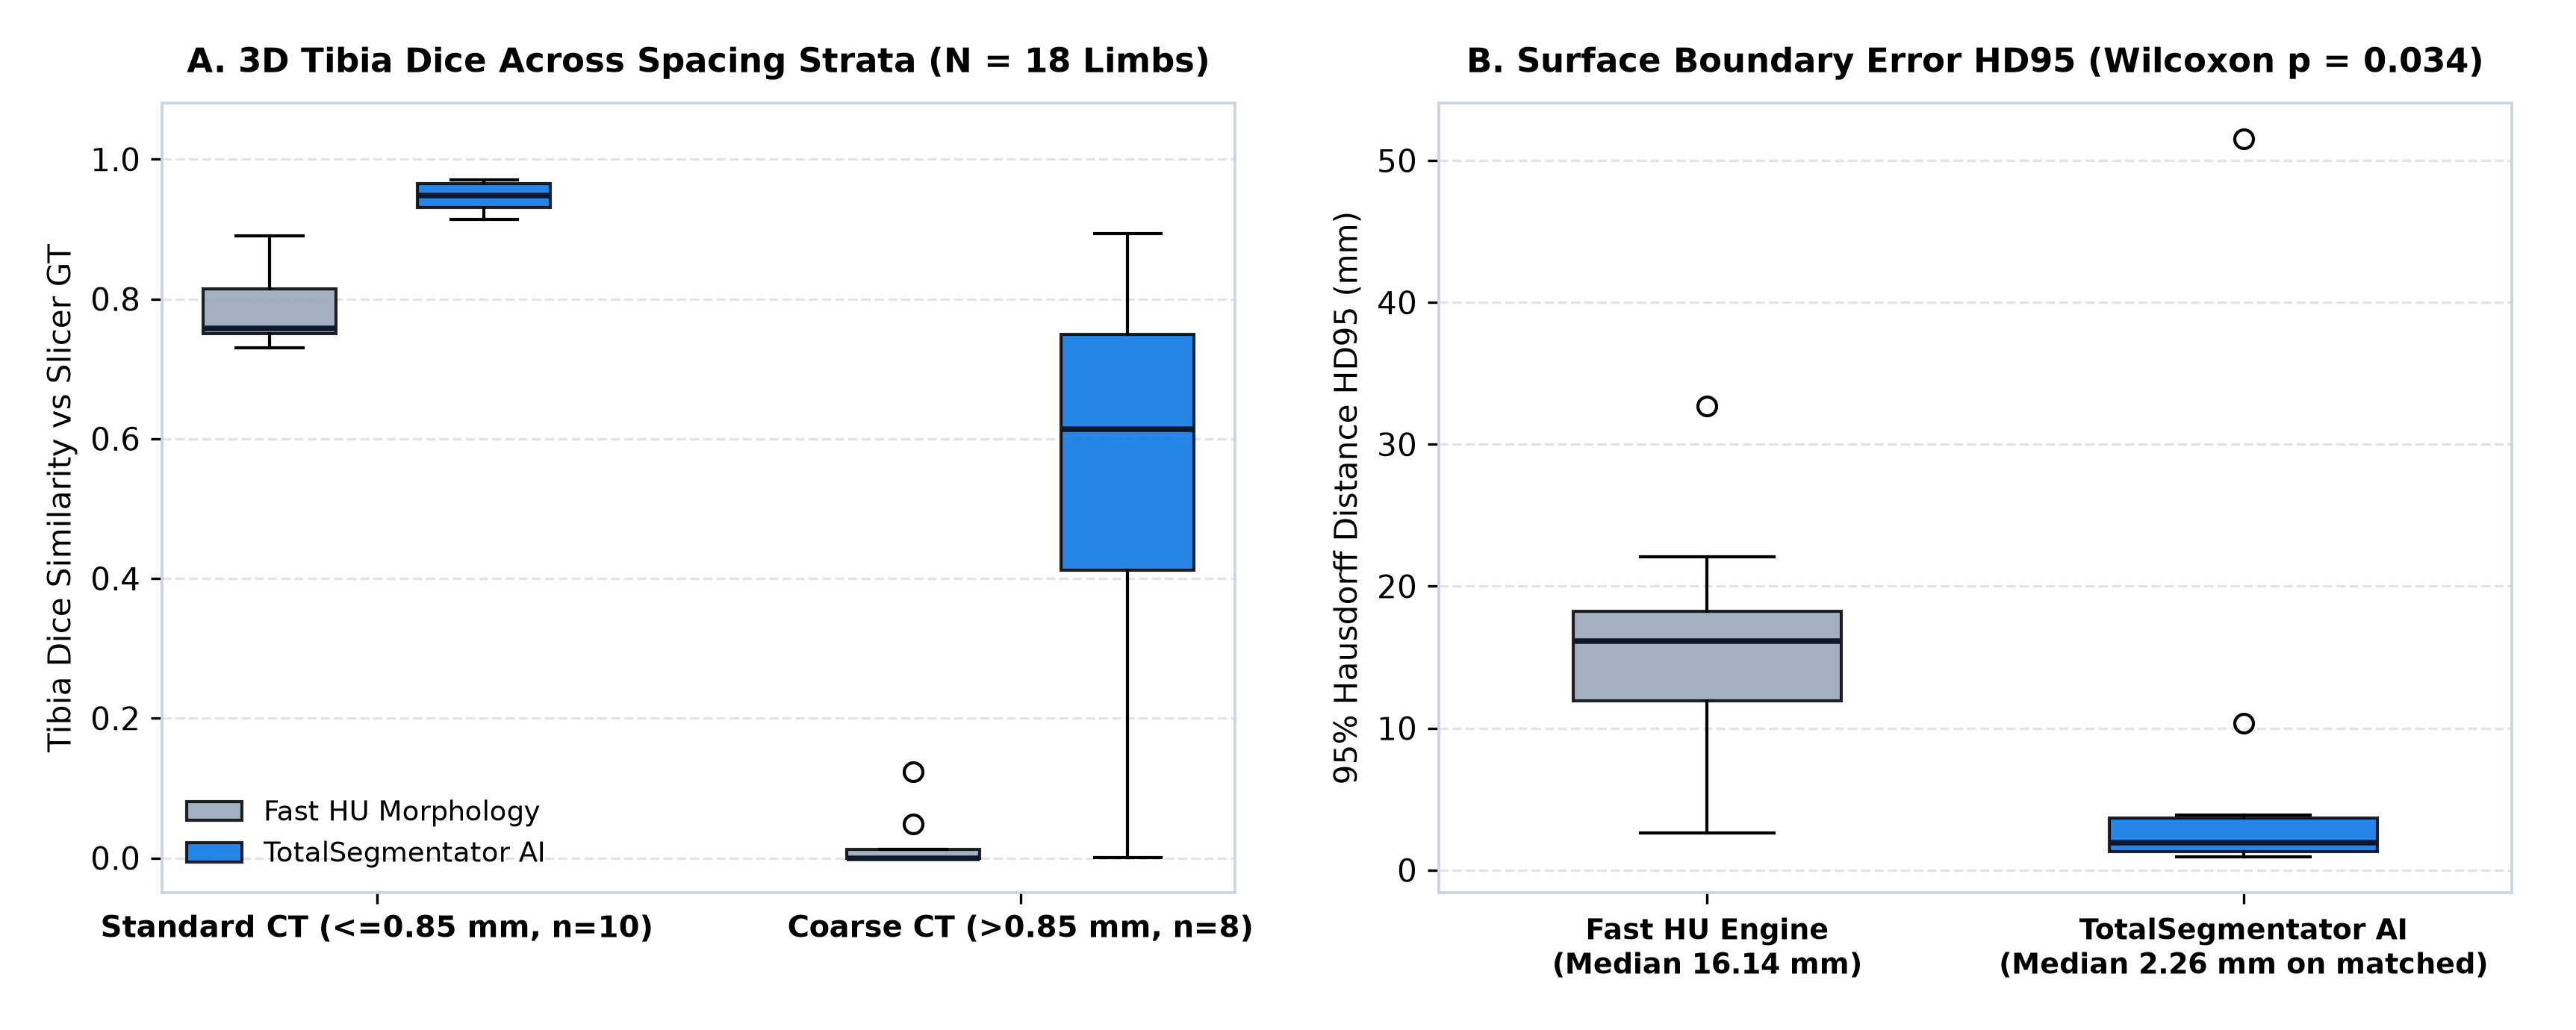
\includegraphics[width=\textwidth]{figures/fig2_vsd18_segmentation.png}
\caption{Paired Tibia Dice and HD95 boundary error across spacing strata ($N=18$ limbs).}
\label{fig:seg}
\end{figure}

\begin{figure}[ht]
\centering
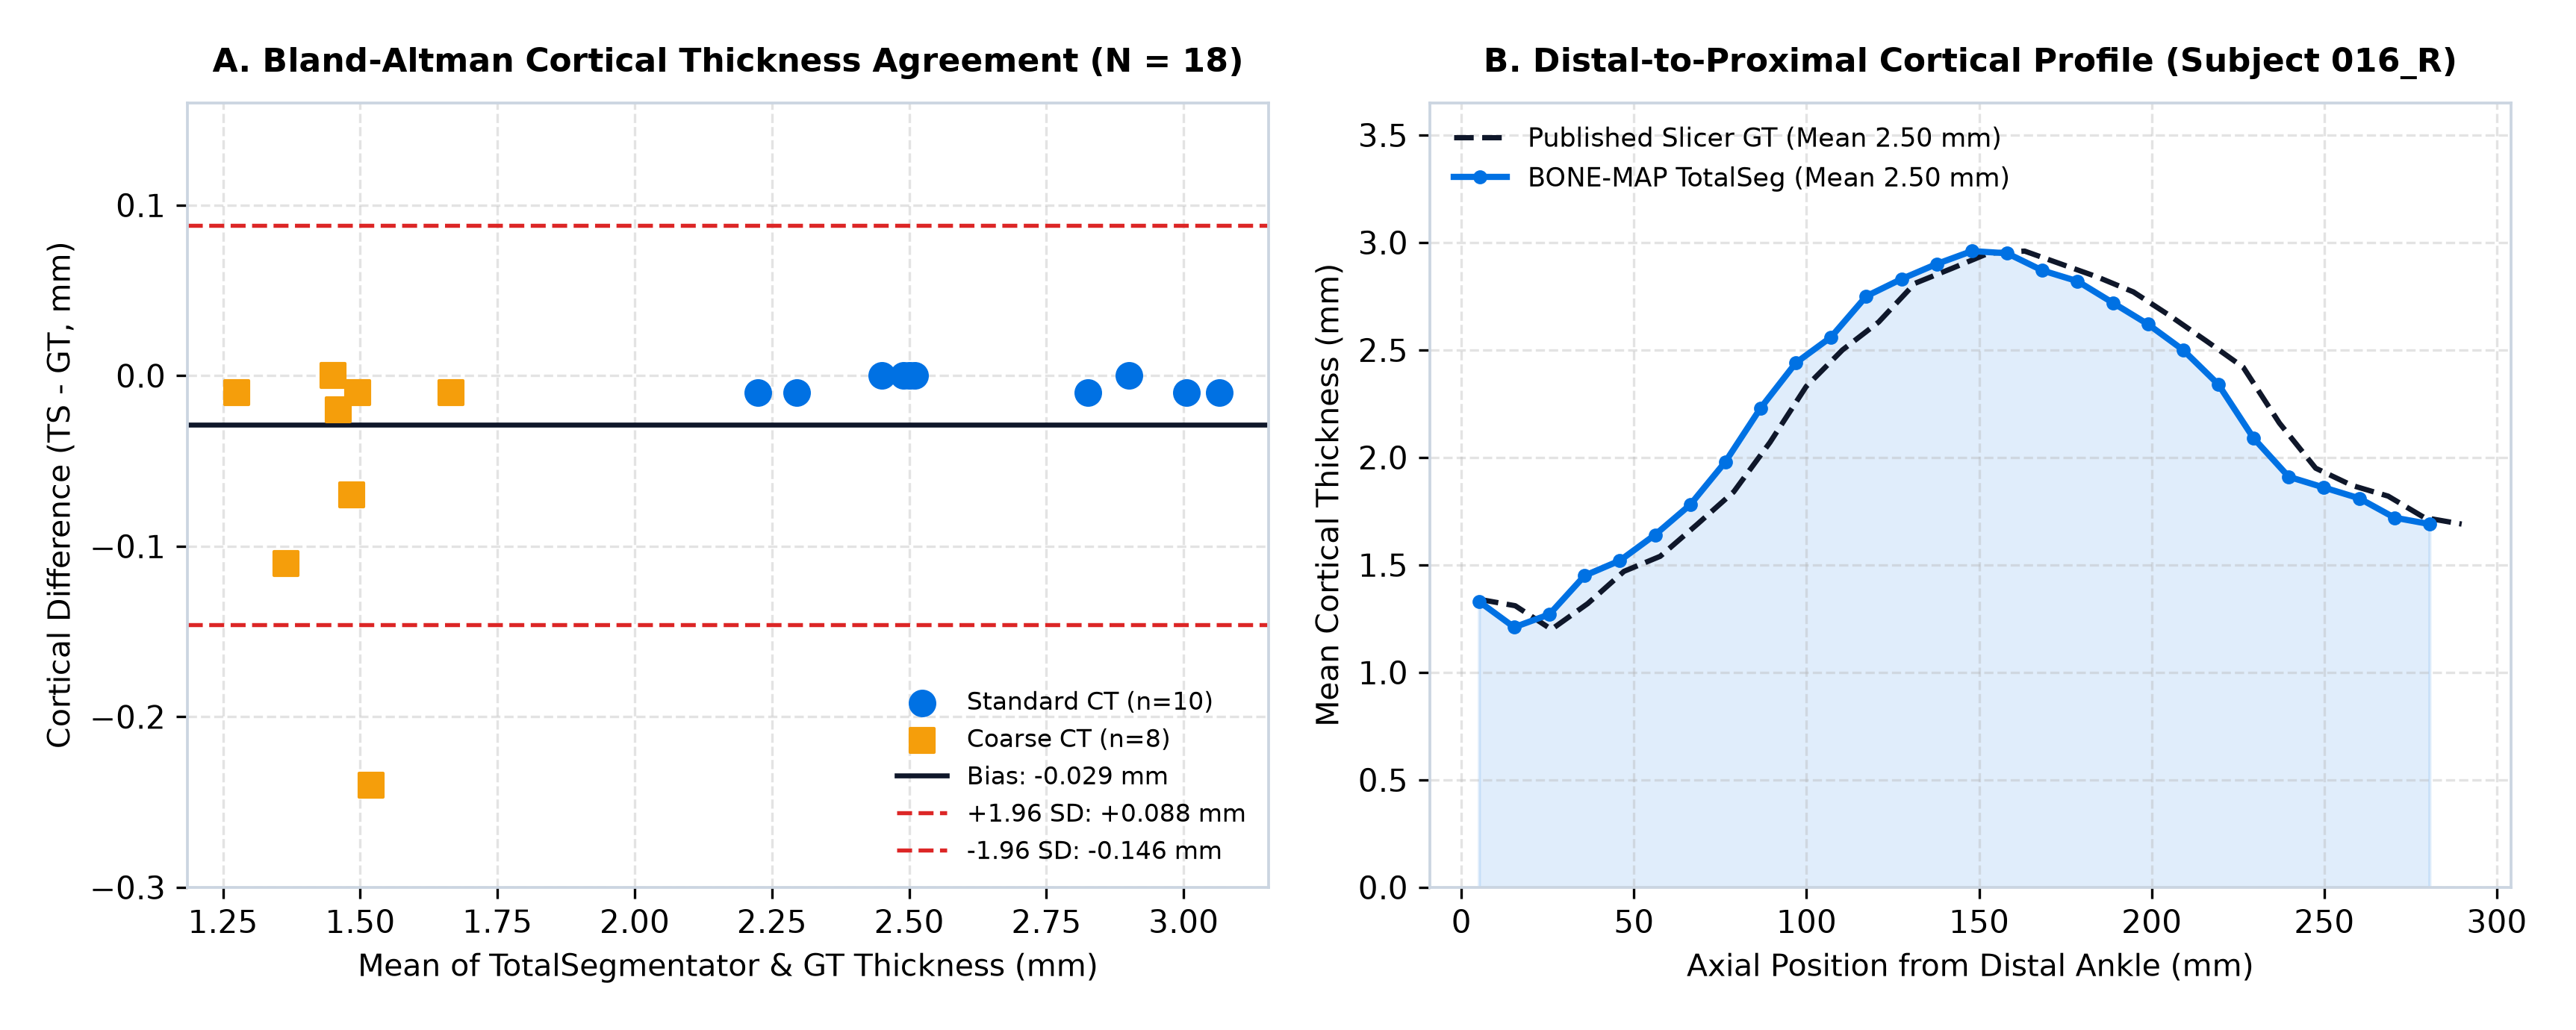
\includegraphics[width=\textwidth]{figures/fig3_bland_altman_cortical.png}
\caption{Bland--Altman cortical thickness agreement ($N=18$) and 28-bin axial profile (Subject 016\_R).}
\label{fig:ba}
\end{figure}

\begin{figure}[ht]
\centering
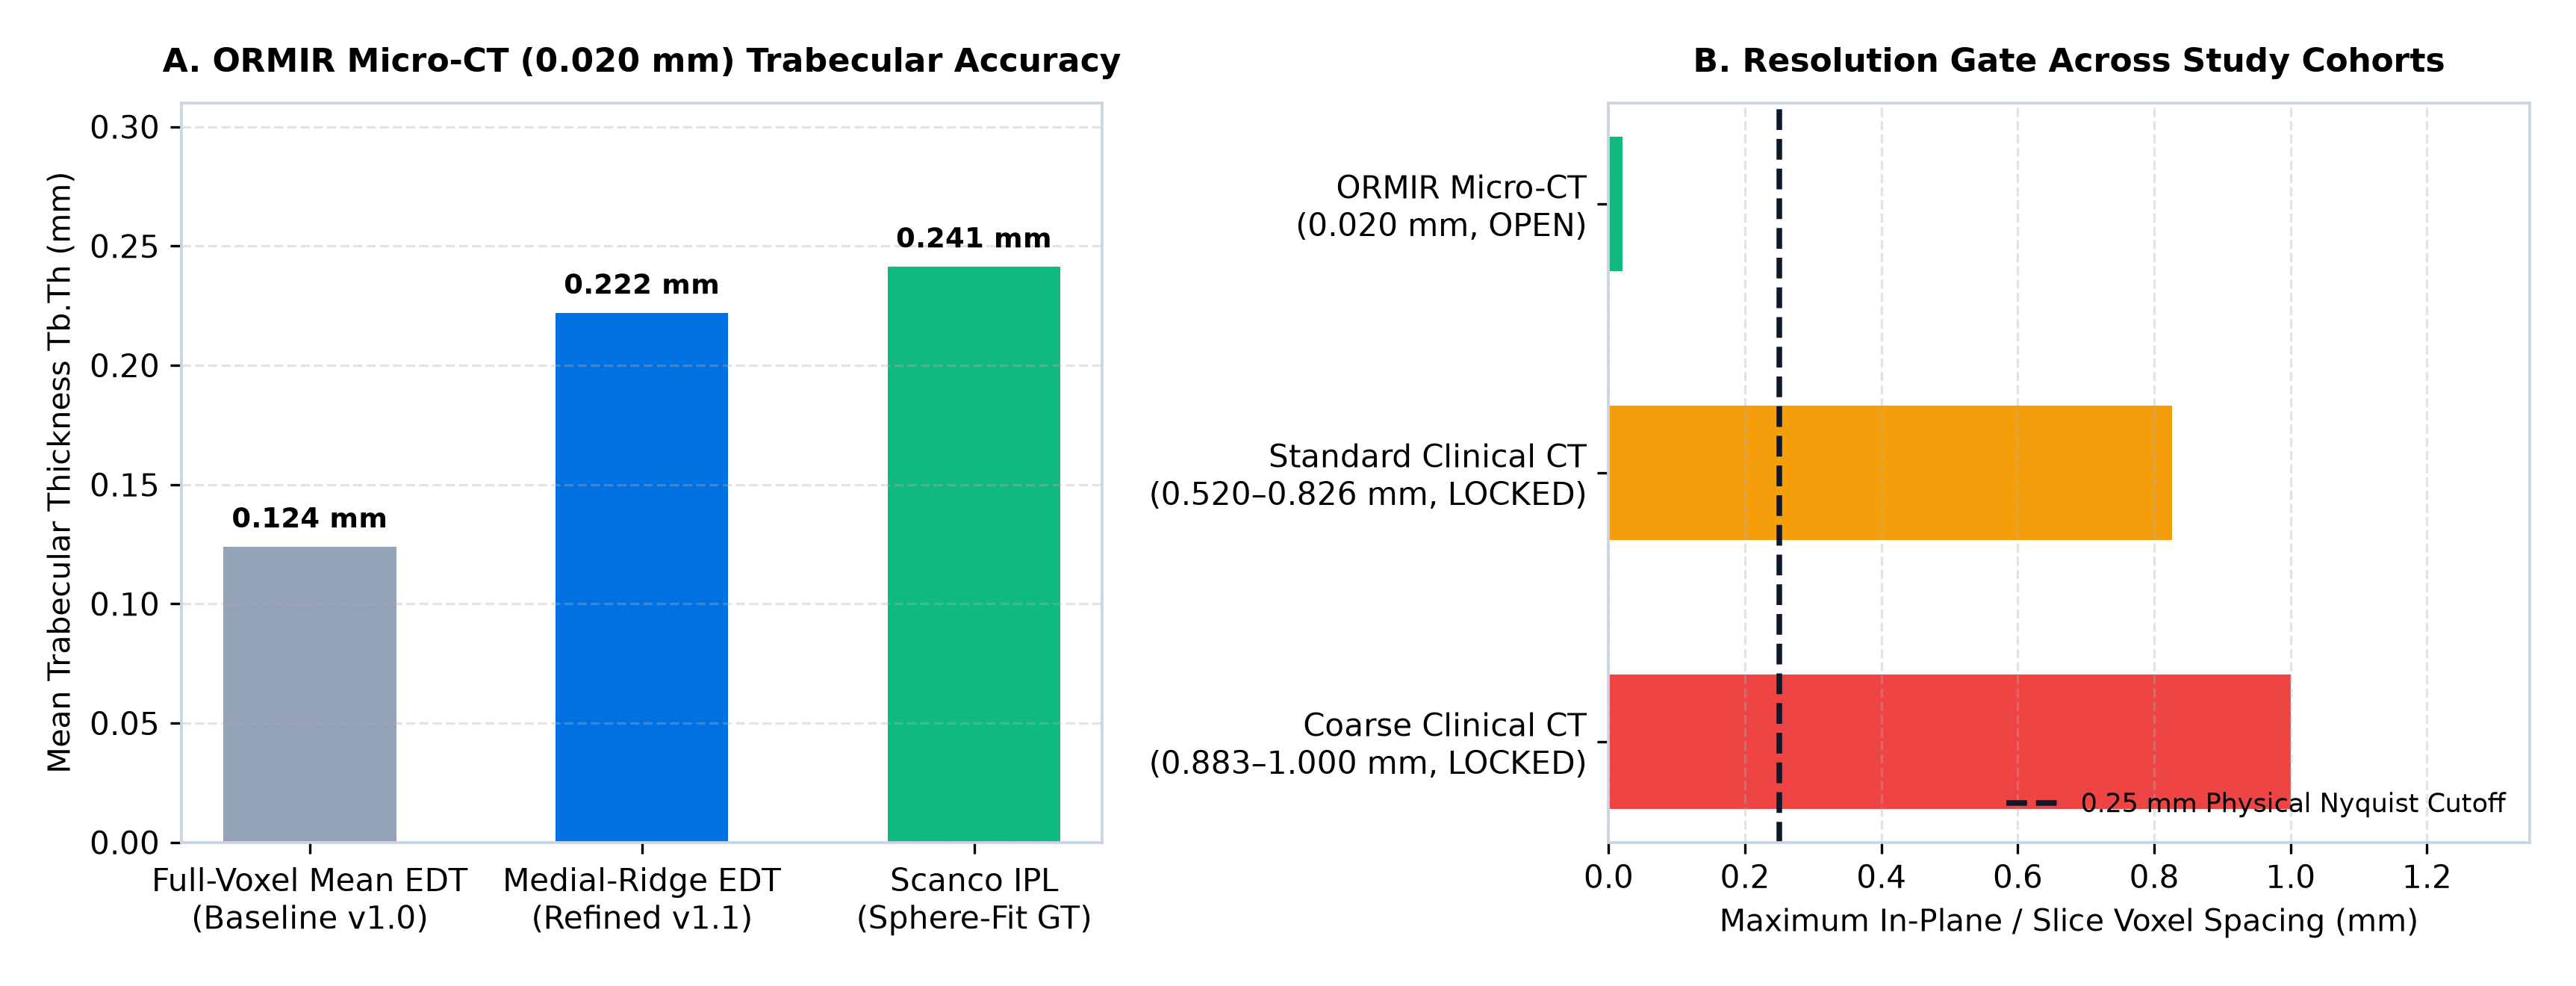
\includegraphics[width=\textwidth]{figures/fig4_resolution_gate_ormir.png}
\caption{Micro-CT trabecular refinement (0.222 vs 0.2414\,mm IPL GT) and resolution gate verification.}
\label{fig:res}
\end{figure}

\begin{figure}[ht]
\centering
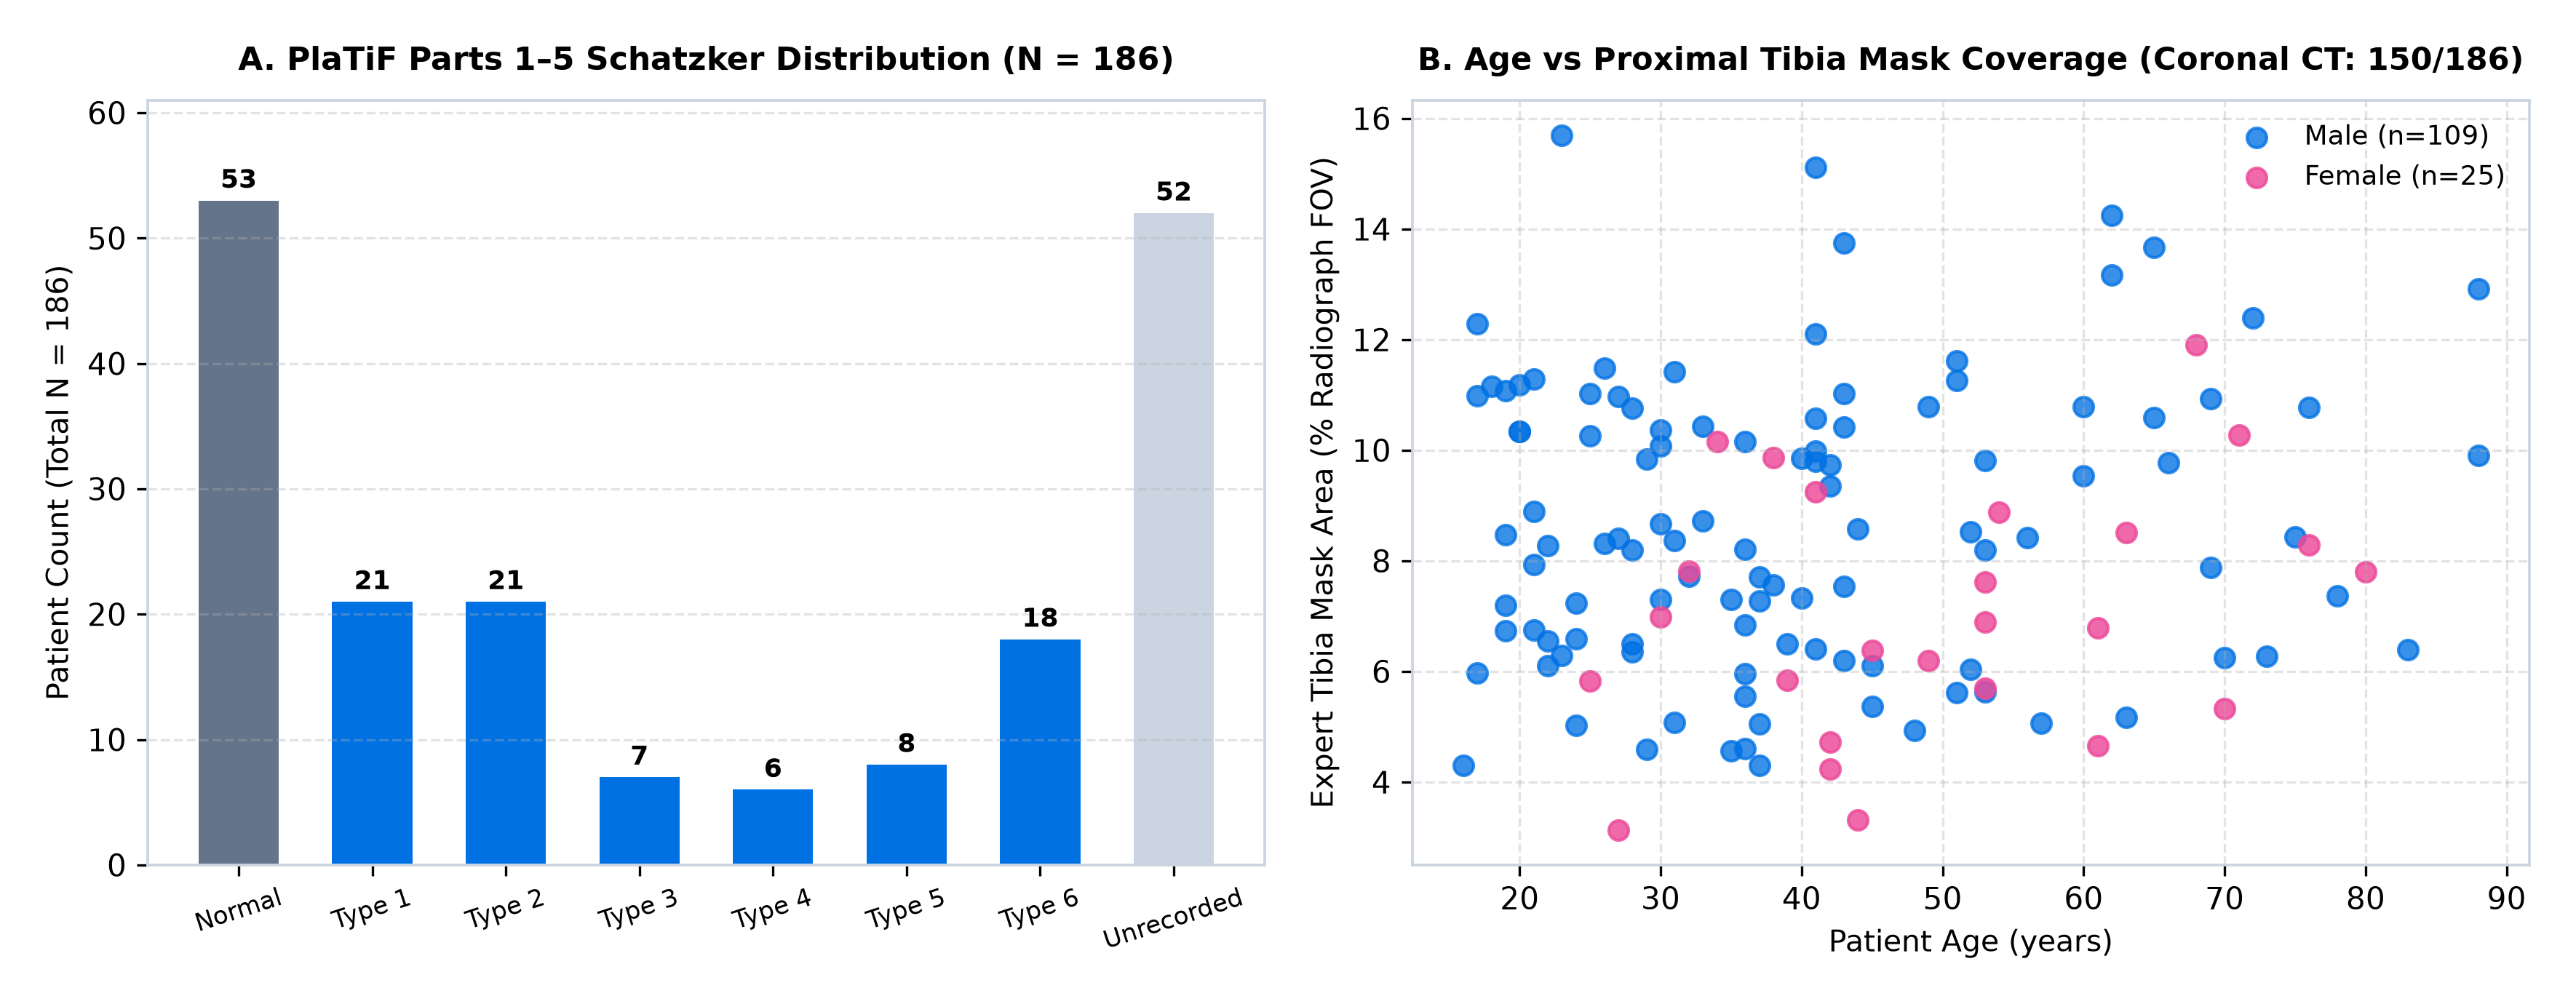
\includegraphics[width=\textwidth]{figures/fig5_platif_186_cohort.png}
\caption{PlaTiF Parts 1--5 cohort ($N=186$) Schatzker distribution and radiograph mask area.}
\label{fig:platif}
\end{figure}

\section{Discussion and Conclusion}
Stratified validation reveals that coarse ($>0.85$\,mm) osteopenic CTs severely degrade single-threshold HU segmentation while deep segmentation maintains sub-0.06\,mm mean cortical thickness accuracy, reinforcing why dual engines, Slicer editability, and explicit Nyquist/BMD locks are essential. Public cohorts lack longitudinal CT-to-physiotherapy follow-up pairs, establishing BONE-MAP as a rigorously verified open-source measurement baseline for prospective clinical studies.

\bibliographystyle{splncs04}
\bibliography{references}
\end{document}
